\chapter{Manos a la obra}
\section{Preparación práctica del ataque} 
%Luego, decir que nos centramos en PSK para el ataque.
Para realizar el ataque, necesitamos una red con protocolo de seguridad WPA2-PSK donde debemos conocer la passphrase o una red sin protocolo de seguridad establecido.

\Nota En caso de tener passphrase y no conocerla, nos veremos obligados a usar el ataque \hyperlink{krack}{KRACK}.


La red inalámbrica que usaremos para emular el ataque, la crearemos con un dispositivo Android, para no interferir con la red principal del edificio\footnote{Salvo que nuestra verdadera intención sea interceptar datos del tráfico que se encuentran en dicha red.}.

Para ello, seguiremos los siguientes pasos:
\begin{enumerate}
	\item Accedemos a ajustes y nos cercioramos de que la conexión Wi-Fi está inhabilitada.
	\begin{center}
			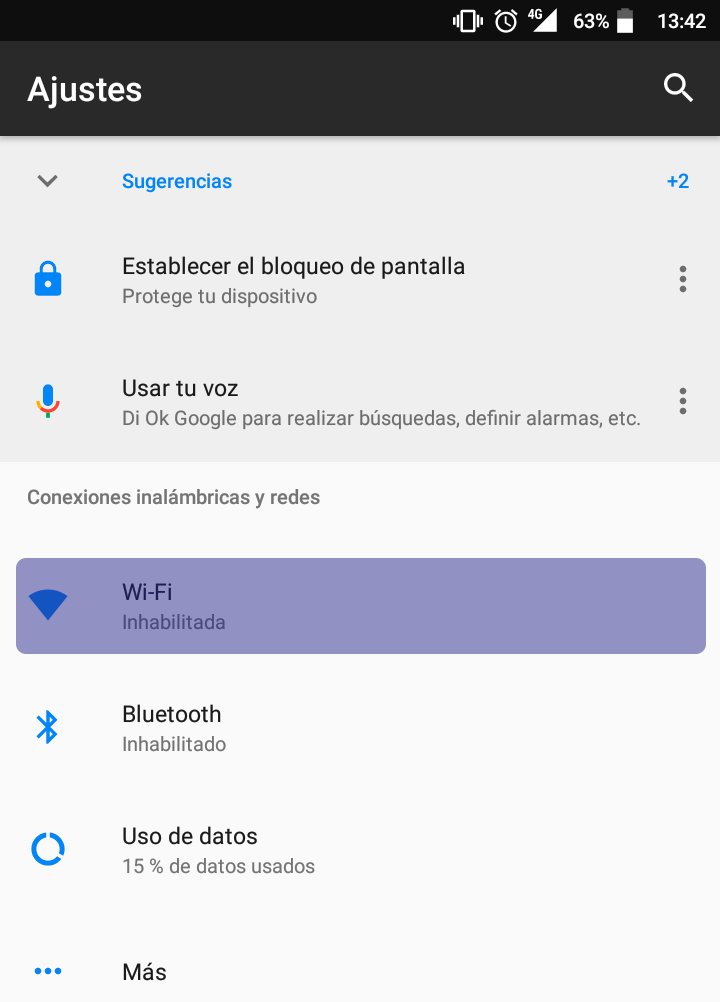
\includegraphics[scale=0.25]{1.png} 
	\end{center}
	\item Entramos en ``Más'' > Anclaje a red y zona Wi-Fi y activamos ``Zona Wi-Fi portátil''.
	\begin{center}
		\begin{tabular}{ c c }
			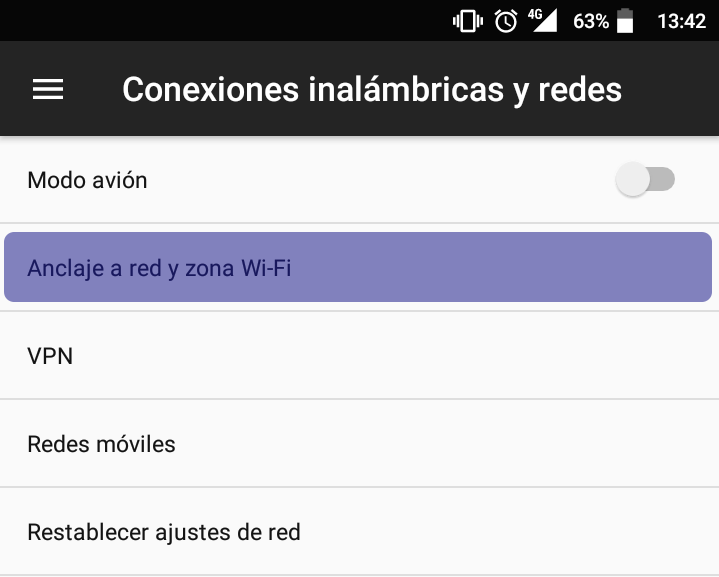
\includegraphics[scale=0.25]{2.png} & 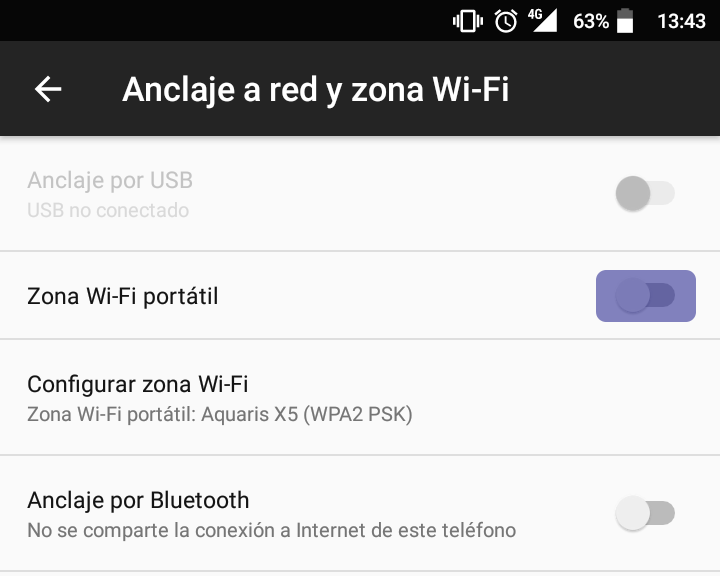
\includegraphics[scale=0.25]{3.png} 
		\end{tabular}		
	\end{center}
	\item Seleccionamos ``Configurar zona Wi-Fi'' y establecemos un nombre, la seguridad que le queramos poner (ninguna o WPA2) y una contraseña.
	\begin{center}
		\begin{tabular}{ c c }
			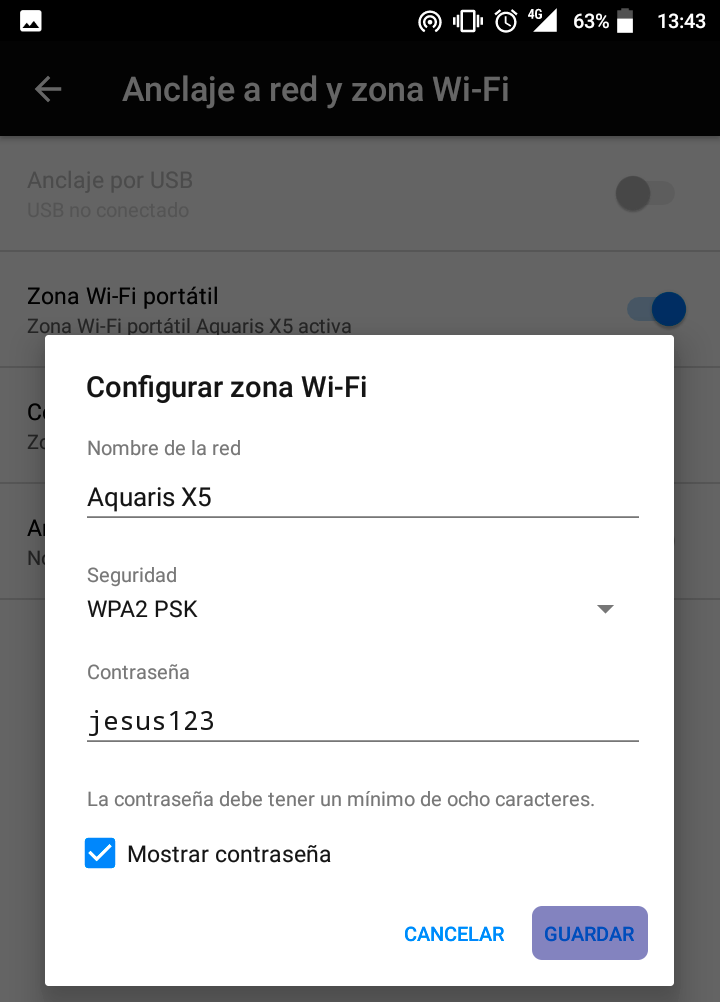
\includegraphics[scale=0.25]{5v2.png} & 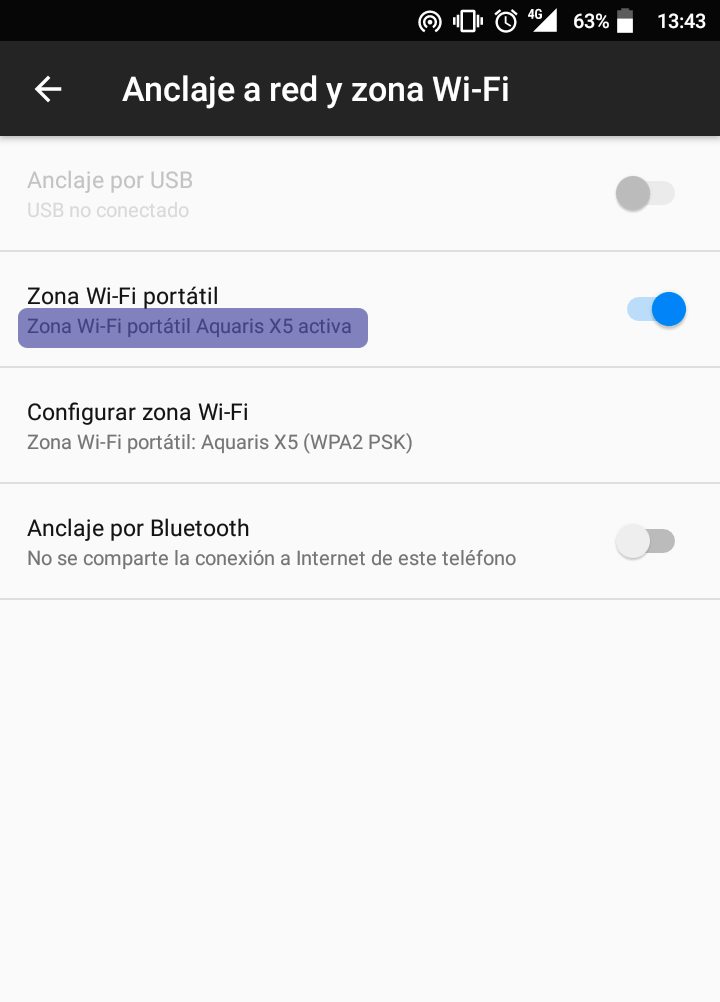
\includegraphics[scale=0.25]{6v2.png} 
		\end{tabular}		
	\end{center}
\end{enumerate}

Llegados a este punto, tendríamos configurada la red inalámbrica en la que vamos a realizar el ataque.

\section{Realización del ataque}
Para la realización del ataque, nuestra víctima tiene que estar conectada a la red inalámbrica en la que vamos a actuar (en nuestro caso, la que acabamos de crear con el dispositivo Android).

\Nota También es posible hacerlo en cualquier red, pero si dicha red tiene muchos hosts conectados, el escaneo de los mismos efectuado más adelante puede tardar demasiado tiempo.

A continuación, lo primero debemos hacer un breve reconocimiento de la red y ver si nuestra víctima está conectada a ella y luego, actuar para sustraerle las credenciales al ingresar en una página con protocolo HTTP donde ha iniciado sesión (para este ejemplo y, como se comentó en la preparación teórica del ataque, se usará la página web \url{http://minecub.es/}.)

\subsection{Reconocimiento de la red}
Para realizar un reconocimiento de la red usaremos lo siguiente:
\begin{itemize}
	\item \textbf{\texttt{ifconfig}:} En caso de no venir instalado (como pasa en Debian 9), instalarlo con \texttt{sudo apt-get install net-tools}.
	\item \textbf{\texttt{nmap}:} En caso de no estar instalado, instalarlo con \texttt{sudo apt-get install nmap}.
\end{itemize}

Una vez contamos con estas dos herramientas seguimos los siguientes pasos:
\begin{enumerate}
	\item Abrimos la terminal y lanzamos la orden \texttt{ifconfig} en modo superusuario, que nos dará información sobre nuestra dirección IP y la máscara de red.
	\begin{center}
		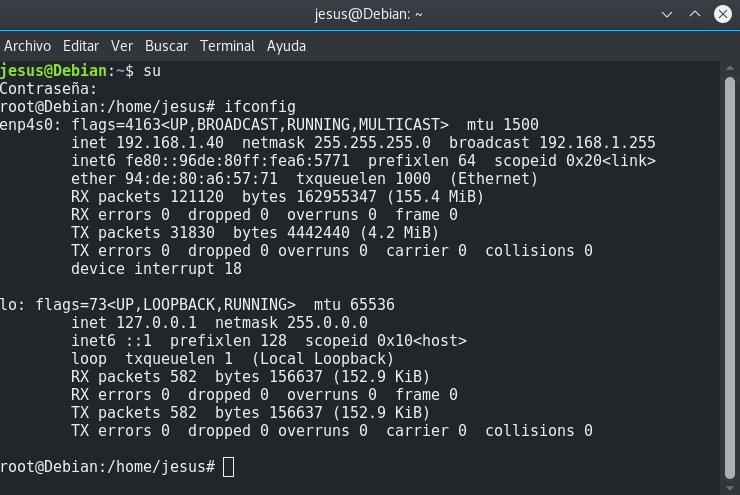
\includegraphics[scale=0.5]{ip.png}
	\end{center}
	Tal como se puede ver en la imagen, la ip de nuestro ordenador es 192.168.1.40 y, según la máscara de red (255.255.255.0) podemos deducir que la ip de la red es 192.168.1.0/24.
	\newpage
	\item En la terminal realizamos un mapeo de la red con nmap dando la orden \texttt{nmap -sP 192.168.1.0/24} como superusuario. La opción \texttt{-sP} le indica a nmap que únicamente realice un descubrimiento de sistemas mediante un sondeo ping, y que luego emita un listado de los equipos que respondieron al mismo. 
	\begin{center}
		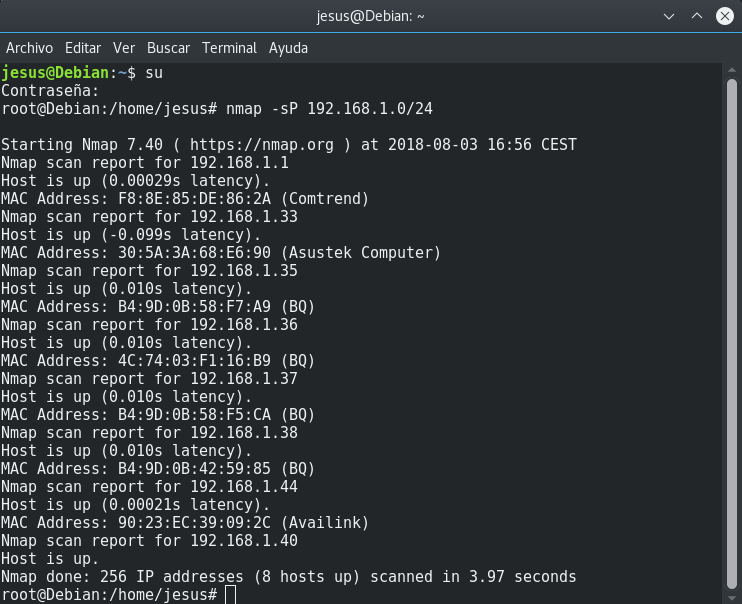
\includegraphics[scale=0.5]{nmap.png}
	\end{center}
	\item Buscamos a nuestra víctima (que en este ejemplo tiene la IP 192.168.1.36 y la MAC 4C:74:03:F1:16:B9) y se encuentra conectado a la red con una latencia de 0.010 segundos tal como podemos ver en la imagen anterior.
\end{enumerate}

\subsection{Atacar a nuestra víctima}
Una vez que tenemos identificada a nuestra víctima, solo tenemos que abrir Ettercap y usando las herramientas que nos ofrece, este ataque se vuelve muy sencillo de realizar.

Para conseguir las credenciales de usuario de nuestra víctima seguiremos los siguientes pasos:
\newpage
\begin{enumerate}
	\item Abrimos Ettercap en modo gráfico y nos dirigimos a la opción ``Sniff'' > ``Unified Sniffing...'' y seleccionamos la interfaz de red que estemos usando.
	\begin{center}
		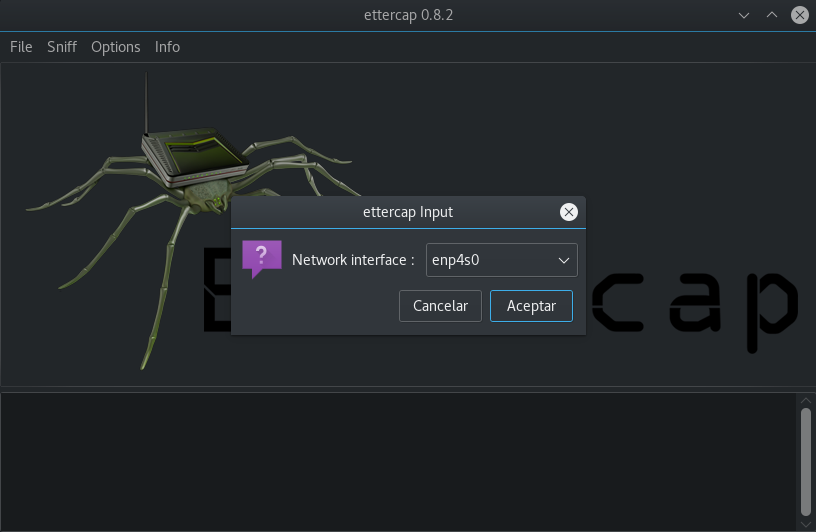
\includegraphics[scale=0.5]{e1.png}
	\end{center}
	\item Seleccionamos la opción ``Hosts'' > ``Scan for hosts''.
	\begin{center}
		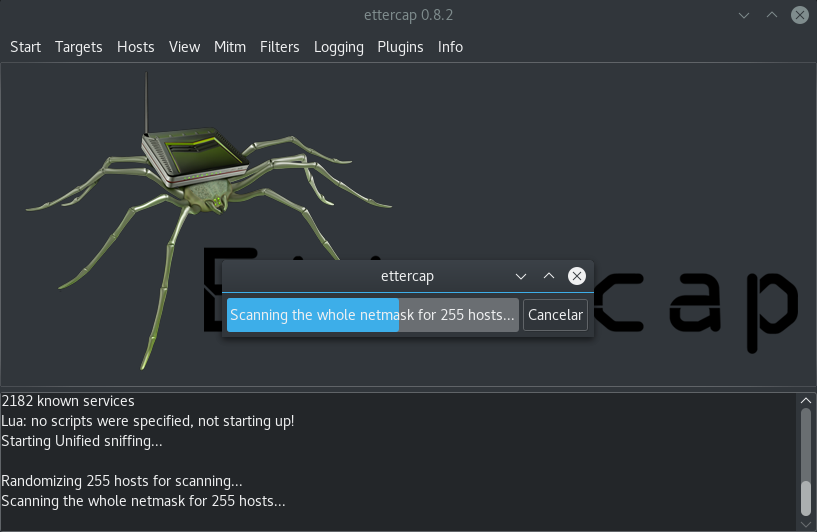
\includegraphics[scale=0.5]{e2.png}
	\end{center}
	\newpage
	\item Seleccionamos la opción ``Hosts'' > ``Hosts list''. Identificamos a nuestra víctima, la seleccionamos y hacemos click en la opción ``Add to Tarjet 1''.
	\begin{center}
		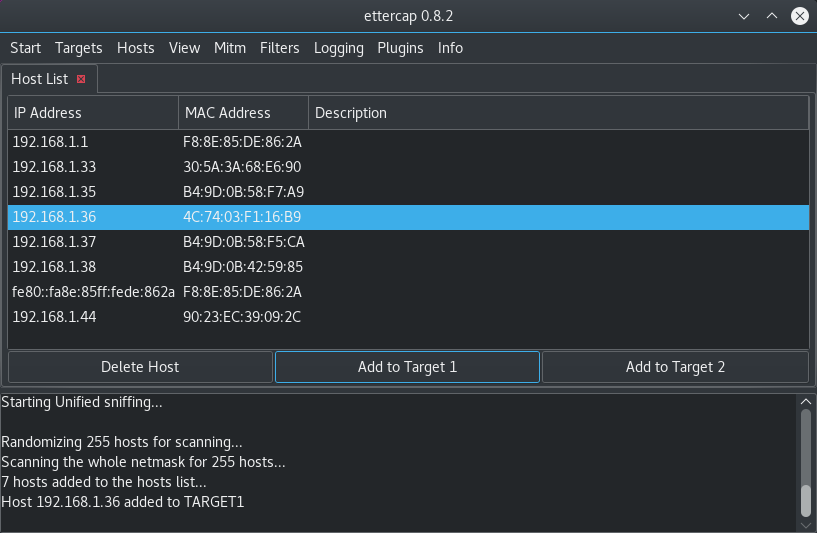
\includegraphics[scale=0.5]{e3.png}
	\end{center}
	\item Seleccionamos la opción ``Mitm'' > ``ARP Poisoning..." y seleccionamos la opción ``Sniff remote conections.''.
	\begin{center}
		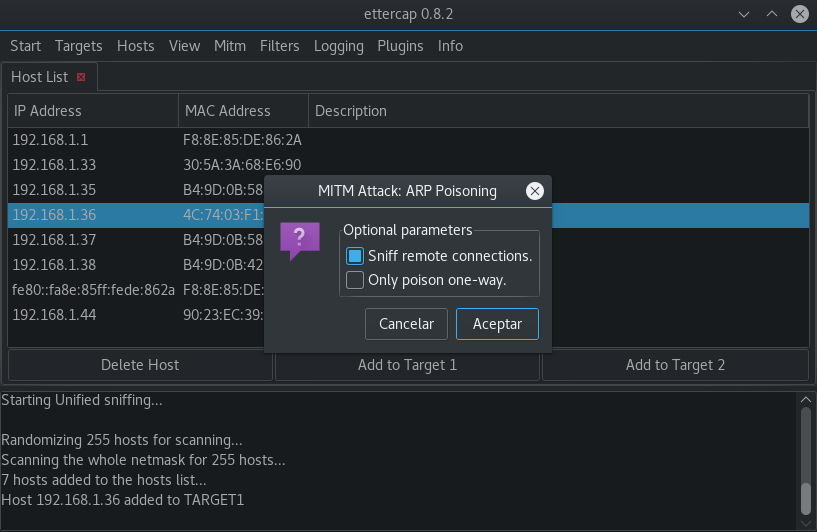
\includegraphics[scale=0.5]{e4.png}
	\end{center}
	\newpage
	\item Seleccionamos la opción ``Start'' > ``Start sniffing'' y una vez que nuestra víctima haya accedido a una página con protocolo HTTP y haya introducido sus credenciales, las obtendremos nosotros instantáneamente en la pequeña consola de Ettercap.
	\begin{center}
		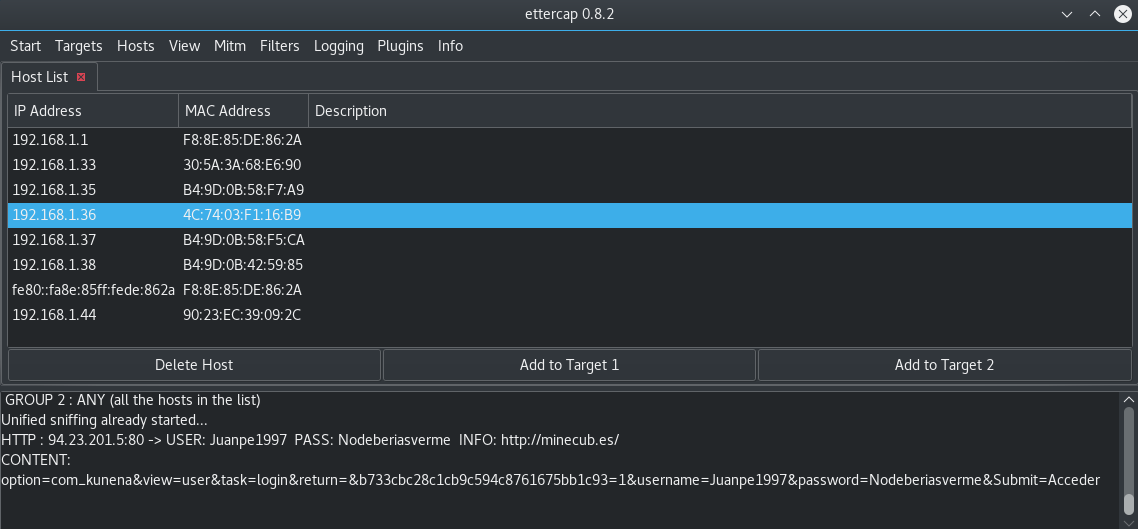
\includegraphics[scale=0.38]{e5.png}
	\end{center}
\end{enumerate}

Una vez hayamos concluido el ataque, seleccionamos la opción ``Start'' > ``Stop sniffing'' y luego ``Start'' > ``Exit'' y se deshace el ARP Poisoning que habíamos establecido antes de realizar el ataque.